%%
%% This is file `sample-manuscript.tex',
%% generated with the docstrip utility.
%%
%% The original source files were:
%%
%% samples.dtx  (with options: `manuscript')
%% 
%% IMPORTANT NOTICE:
%% 
%% For the copyright see the source file.
%% 
%% Any modified versions of this file must be renamed
%% with new filenames distinct from sample-manuscript.tex.
%% 
%% For distribution of the original source see the terms
%% for copying and modification in the file samples.dtx.
%% 
%% This generated file may be distributed as long as the
%% original source files, as listed above, are part of the
%% same distribution. (The sources need not necessarily be
%% in the same archive or directory.)
%%
%% The first command in your LaTeX source must be the \documentclass command.
%%%% Small single column format, used for CIE, CSUR, DTRAP, JACM, JDIQ, JEA, JERIC, JETC, PACMCGIT, TAAS, TACCESS, TACO, TALG, TALLIP (formerly TALIP), TCPS, TDSCI, TEAC, TECS, TELO, THRI, TIIS, TIOT, TISSEC, TIST, TKDD, TMIS, TOCE, TOCHI, TOCL, TOCS, TOCT, TODAES, TODS, TOIS, TOIT, TOMACS, TOMM (formerly TOMCCAP), TOMPECS, TOMS, TOPC, TOPLAS, TOPS, TOS, TOSEM, TOSN, TQC, TRETS, TSAS, TSC, TSLP, TWEB.
% \documentclass[acmsmall]{acmart}

%%%% Large single column format, used for IMWUT, JOCCH, PACMPL, POMACS, TAP, PACMHCI
% \documentclass[acmlarge,screen]{acmart}

%%%% Large double column format, used for TOG
% \documentclass[acmtog, authorversion]{acmart}

%%%% Generic manuscript mode, required for submission
%%%% and peer review
\documentclass[manuscript,screen]{acmart}

%%
%% \BibTeX command to typeset BibTeX logo in the docs
\AtBeginDocument{%
  \providecommand\BibTeX{{%
    \normalfont B\kern-0.5em{\scshape i\kern-0.25em b}\kern-0.8em\TeX}}}

%% Rights management information.  This information is sent to you
%% when you complete the rights form.  These commands have SAMPLE
%% values in them; it is your responsibility as an author to replace
%% the commands and values with those provided to you when you
%% complete the rights form.
%\setcopyright{acmcopyright}
\copyrightyear{2020}
%\acmYear{2020}
%\acmDOI{10.1145/1122445.1122456}

%% These commands are for a PROCEEDINGS abstract or paper.
%\acmConference[Woodstock '18]{Woodstock '18: ACM Symposium on Neural
 % Gaze Detection}{June 03--05, 2018}{Woodstock, NY}
%\acmBooktitle{Woodstock '18: ACM Symposium on Neural Gaze Detection,
 % June 03--05, 2018, Woodstock, NY}
%\acmPrice{15.00}
%\acmISBN{978-1-4503-XXXX-X/18/06}

%%
%% end of the preamble, start of the body of the document source.
\begin{document}

%%
%% The "title" command has an optional parameter,
%% allowing the author to define a "short title" to be used in page headers.
\title{Learning Music with Adaptive Visualizations}

%%
%% The "author" command and its associated commands are used to define
%% the authors and their affiliations.
%% Of note is the shared affiliation of the first two authors, and the
%% "authornote" and "authornotemark" commands
%% used to denote shared contribution to the research.
\author{Jordan Aiko Deja}
%\authornote{Both authors contributed equally to this research.}
\email{jordan.deja@famnit.upr.si}
\orcid{1234-5678-9012}
\affiliation{%
  \institution{University of Primorska}
  \city{Koper}
  \country{Slovenia}
  \postcode{6000}
}

%\author{Matjaž Kljun and Klen Čopič Pucihar}
%\affiliation{%
%  \institution{Advisors}
%  \city{Koper}
 % \postcode{6000}}
%\email{\{matjaz.kljun, klen.copic\}@famnit.upr.si}

%\author{Klen Čopič Pucihar}
%\affiliation{%
%  \institution{University of Primorska}
 % \city{Koper}
  %\country{Slovenia}
  %\postcode{6000}}
%\email{klen.copic@famnit.upr.si}

%%
%% By default, the full list of authors will be used in the page
%% headers. Often, this list is too long, and will overlap
%% other information printed in the page headers. This command allows
%% the author to define a more concise list
%% of authors' names for this purpose.
\renewcommand{\shortauthors}{Deja, et al.}
%%
%% The abstract is a short summary of the work to be presented in the
%% article.
\begin{abstract}
\textbf{Abstract:} Learning a musical instrument is hard; thus many approaches have been introduced to support novice players. In recent years, a number of prototypes have been introduced using AR visualizations to support novices. While music has a temporal component, previous AR piano prototypes have not incorporated this approach. In this research, we investigate how the temporal component and psycho cognitive responses have an effect on the training of piano learners. We will build an AR projection system to support piano learning using adaptive visualizations. Our study will involve participants (novices and experts) that will train using our AR piano prototype. This will allow us to analyze their training patterns and build spatiotemporal and cognitive models. These models can then be used to build adaptive visualizations and discover affordances that improve the experiences of piano learners. 
\end{abstract}
%%
%% The code below is generated by the tool at http://dl.acm.org/ccs.cfm.
%% Please copy and paste the code instead of the example below.
%%
\begin{CCSXML}
<ccs2012>
   <concept>
       <concept_id>10003120.10003121.10003126</concept_id>
       <concept_desc>Human-centered computing~HCI theory, concepts and models</concept_desc>
       <concept_significance>500</concept_significance>
       </concept>
   <concept>
       <concept_id>10003120.10003145</concept_id>
       <concept_desc>Human-centered computing~Visualization</concept_desc>
       <concept_significance>100</concept_significance>
       </concept>
 </ccs2012>
\end{CCSXML}
\ccsdesc[500]{Human-centered computing~HCI theory, concepts and models}
\ccsdesc[100]{Human-centered computing~Visualization}
%%
%% Keywords. The author(s) should pick words that accurately describe
%% the work being presented. Separate the keywords with commas.
\keywords{extended reality, spatiotemporal pointing, piano, music teaching ystems}
%%
%% This command processes the author and affiliation and title
%% information and builds the first part of the formatted document.
\maketitle

\section{Introduction}
The process of learning a musical instrument is usually tedious and repetitive. It requires keen hand-eye coordination, mastery of complex music sheet notation and more importantly, hours of continuous practice. Having a tutor or a maestro usually provides an improved learning experience since novices can receive immediate feedback during their practice. However, tutors are usually expensive and are not always readily-available. The learning process varies as well depending on the type of music instrument and its availability. Guitars are usually portable but may not be very comfortable to use if not equipped with the right strings. Pianos, are stationary instruments that are comfortable to use but are mostly-expensive and therefore are usually rare in terms of convenience towards practice. All of these are some of the known factors that make learning a music instrument a challenging task.\\

Several technology interventions have been introduced to assist in one or some of the pain points in learning a music instrument. The reviews done by \citet{fober2007vemus} and \citet{daniel2006exploring} covered different technologies to assist music learning ranging from prototype design, ergonomics, groupware and many others. The studies made by \citet{creech2010learning} and \citet{cope1997cultural} considered cultural and societal factors along with these technologies. More recently, Augmented Reality (AR) has been introduced as substitute of tutors for music instrument learners. This approach became popular that it lead to a rise of AR prototypes being  developed and published  \cite{santos2013augmented}. Most of the innovations introduced by these AR piano systems are either in prototype design \cite{barakonyi2005augmented, huang2011piano}, learning modes \cite{rogers2014piano} or visualizations \cite{chow2013music}. While these AR prototypes have reported improvements in the learning process of novices, no prototype (at the best of our knowledge) consider music temporality in the design of adaptive visualizations. \\

Music has been known to have a temporal component \cite{lippman1984progressive}. This has been observed to have an effect among listener experiences. In the work of \citet{large2002perceiving}, small, systematic temporal irregularities have led to improvements in tracking during musical performances. While this work has been observed on traditional setups, these have yet to be explored in AR piano prototypes. Oscillations, rhythms and many other factors describe the temporal component in music. In the context of AR visualizations, users having to press the right key at the right time given a visual stimuli would then describe the spatiotemporal applicability of music.\\

During the music learning process, novices usually experience being overwhelmed. The work of \citet{klepsch2017development} have measured the cognitive load of learners and how the amount of visual stimuli may potentially overwhelm the user. \citet{yuksel2016learn} through their study, have introduced an adaptive learning interface that adjusts based on the current brain state of the learner. The work of \citet{rikers2004cognitive} have explored how adjustments in cognitive load assists in developing expertise and how these systems can be designed to support them. While these studies have supported novice music learning, the temporal component of music has yet to be integrated as well.\\

This work will focus on integrating the spatiotemporal component of music and the cognitive load of users while using AR prototypes. It builds on the spatiotemporal modelling work by \citet{lee2016modelling, lee2017boxer, kim2018impact, liao2020button} where they have modelled and predicted error rates of users doing spatiotemporal tasks such as batting a virtual baseball, clicking a moving and tricky target, and pressing a tactile button at the right time. It also considers the user's internal time-keeping mechanism given an external stimulus following the WK model \cite{wing1973response, wing1973timing}; how Fitts' Index of Difficulty (ID) explains the quality of pointing performance \cite{mackenzie1992extending, park2020intermittent} and the effect of visualizations in relation with Cognitive Load Theory (CLT) \cite{klepsch2017development}.\\

% Our work will focus on investigating spatiotemporal pointing by exploring augmented reality (AR) music teaching systems - specifically a piano teaching system. Spatiotemporal interactions in immersive environments such as virtual, augmented and mixed reality systems (umbrella term for these is extended reality (XR)) refer to a range of user activities that users need to perform in relation to both time and space. Temporal interaction requires users’ actions within a particular time window in response to an event taking place. For example, several recent studies have explored temporal pointing \cite{lee2016modelling} defined as interaction in which users need to provide a discrete input (e.g., button press), with no or negligible spatial aiming demand (the finger is on the button) in a particular time window (usually very short). Spatial interaction requires users to complete an action at a particular place in space. In contrast to temporal pointing, spatial pointing requires users to aim at a fixed or moving target in space while time is not predefined (e.g. just as quickly as possible). As such, spatiotemporal pointing combines these two principles and is referred to as the user action in an immersive environment as a response to a temporarily available digital stimulus. Examples of spatiotemporal interactions include batting a virtual baseball in a XR environment or hitting the right keys at the right time in an XR piano teaching system. In both examples users need to point to a precise location (hitting the ball with a controller representing the virtual bat or pressing the piano key) at the right time. \\

%To be able to complete such spatiotemporal pointing \cite{lee2016modelling}, users have an internal time-keeping mechanism to synchronise their movements to an external stimulus according to the WK model \cite{wing1973response}. Additionally, a response-execution stage that allows the user to process input-stimulus and output-actions, is also needed \cite{wing1973timing}. Other studies have focused on (i) investigating and understanding human cognitive load \cite{radu2009augmented}, (ii) improving the accuracy in the rendering of visual elements (which is also referred to as spatial registration \cite{zheng2013general}), and (iii) discovering novel approaches to minimise latency of visualising overlaying digital visualisations \cite{serafin2017considerations}. \\

%Innovations in spatiotemporal interactions also directly contribute to computational human-computer interaction (HCI). The concept of computational HCI considers usage of explicit mathematical models of user-system behavior in order to influence, automate and improve the design process of a system. For example, the collected user data can directly feed back into a model, improving the behaviour of the targets of spatiotemporal interaction. 

%Since AR environments present an ideal space to investigate spatiotemporal pointing, we push our contributions further by incorporating techniques in computational HCI. Several formative studies have focused on modelling, predicting, and simulating action and reaction in such environments. These studies have contributed to understanding of (1) how objects move and collide in virtual spaces \cite{lee2017boxer}, (2) how users respond to these objects \cite{lee2016modelling} and (3) how we can foster design affordances that improve their performance \cite{rogers2014piano}.\\

Since AR environments present an ideal space to investigate spatiotemporal interactions and cognitive load modelling, our contributions benefit from integrating these two approaches. We will build an AR piano projection system to support piano learning following these two approaches. We present \textit{P.I.A.N.O. 2.0} inspired and built on top of the work by \citet{rogers2014piano}. In this prototype, we will have adaptive visualizations that take into account both the spatiotemporal data and cognitive load of users. Participants will be invited to train with our AR piano prototype where we shall observe its effect to the long term piano learning experiences.\\

In this document, we reviewed related work on spatiotemporal modeling and relevant AR piano systems as found in Section \ref{sec:rrl}. Following this, we described a plan (in Section \ref{sec:plan}) on how we intend to achieve our target contributions stated in Section \ref{sec:contri}. \\

%Several AR piano systems have been built with augmented and virtual reality as a medium for innovation by overlaying augmented time-specific visualisations over piano keys to improve music learning experiences \cite{rogers2014piano, sun2018mr, birhanu2017keynvision}. However, cognitive load and user response times have not been observed and taken into account. Moreover, these prototypes were not based on the pre-built spatiotemporal pointing models. Our research will fill this gap by designing adaptive visualisations based on the pre-built models of spatiotemporal pointing data and cognitive load. 


\section{Related Work}
\label{sec:rrl}
This section will discuss studies on spatial and temporal interactions on screen and in extended reality (XR) environments followed by the section describing AR piano systems. 

\subsection{Studies on modeling spatiotemporal interactions}
Here we present a few studies in temporal and spatiotemporal pointing and error predicting models. 

\begin{figure}[t]
\centering
 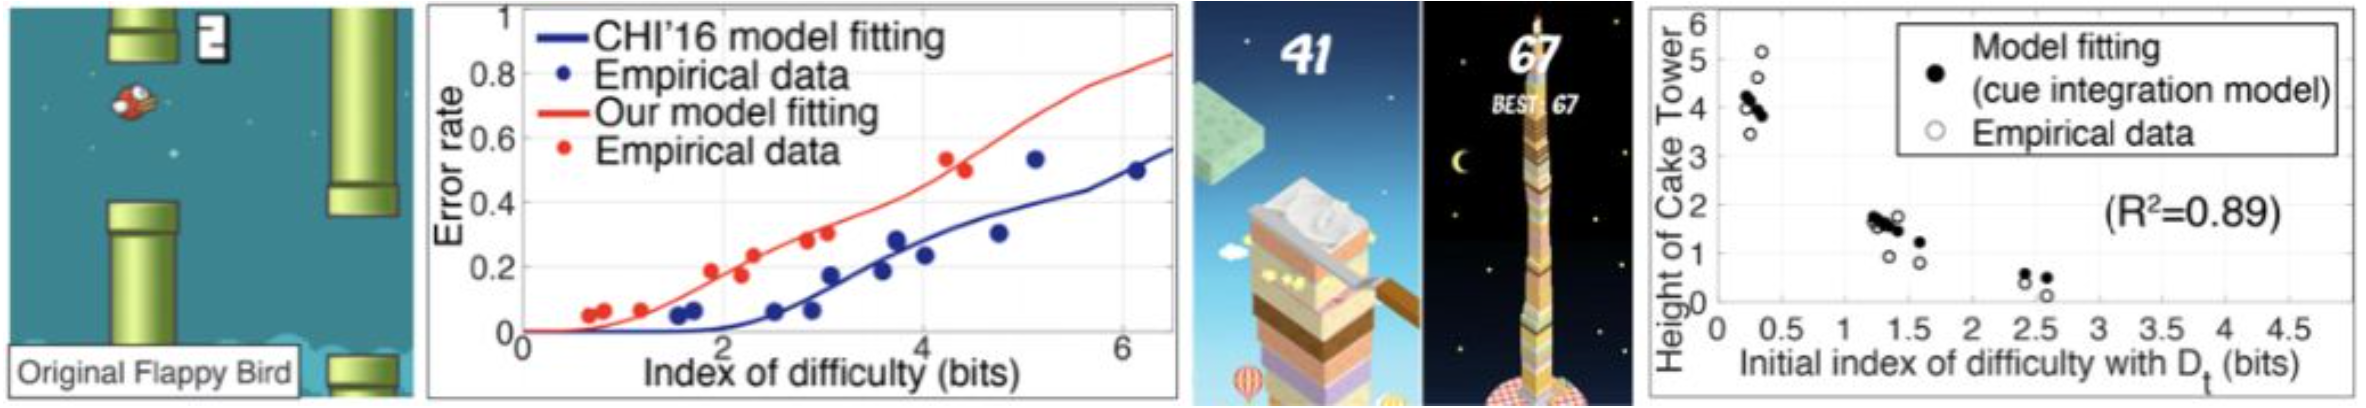
\includegraphics[width=12cm]{figures/flappybird.png}
    \caption{Temporal pointing models could predict player scores and error rates for one-button games such as Flappy Bird (left) and Cake Tower (right).
    }\label{fig:flappybird}
\end{figure}

\begin{itemize}
\item \citet{lee2016modelling} and \citet{lee2018moving} built models to predict players’ performance and error rates in some real-time games that are played with a single button — temporal pointing. Their model could successfully predict the players’ performance while playing popular games such as Flappy Bird and Cake Tower (\ref{fig:flappybird}). The presented model can be applied to adaptively change a game’s difficulty level by changing latency or speed of moving objects). 
\item The study of \citet{lee2017boxer}, investigated collision events of a hand with a virtual object by throwing, pushing or pulling it. In their prototype called Boxer, users received a salient sensory feedback on their palm when a pointer (palm) made a contact with a moving virtual object (a virtual ball). The feedback was triggered when the pointer reached a minimum speed after the collision. The researchers compared this spatiotemporal pointing with a temporal pointing (just pressing a button) presented in the study described before. Based on their findings, spatial precision in collisions improved by 26.7\%. It was also reported that accuracy can be compromised under specific task conditions. Their study also reported that there were no observed differences in temporal precision.
\item The work of \citet{kim2018impact} presented an activation technique called impact activation (IA). This describes the point where a button is activated at its maximal impact point. Based on their findings, IA as a technique is most useful during particularly-rapid repetitive button pressing activities, which are usually observed in games and music applications. While their study focused more on rapid button pressing, their findings were able to report on user’s timing accuracy and how they improved significantly by using IA. The proposed technique can be implemented in modern push-button setups that generate a continuous signal. In music teaching systems, pressing the piano key resembles an action of pressing a button. Users pressing on a setup like a piano teaching system may potentially take advantage from accuracy improvements that use impact activation.
\item The work of \citet{park2020intermittent} designed an Intermittent Click Planning (ICP) model on moving targets. The study aims to understand and model \textit{submovements} and the planning process that users usually undertake before clicking a moving target. This ICP model predicted the error rates between gamers and non-gamers when trying to click moving and tricky targets. Based on their findings, gamers and more experienced users performed better (with reduced errors) than their non gamer counterparts. The ICP model was also successfully able to predict these errors. While this study focused on clicking a moving target, the model and the internal time-keeping mechanism behind the click planning can be used to understand spatiotemporal interactions of piano novices in AR systems as well. 
\end{itemize}

\begin{figure}[t]
\centering
 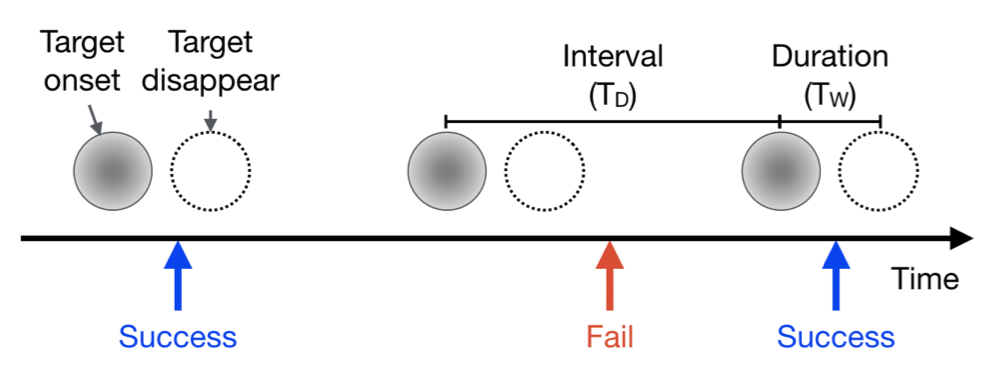
\includegraphics[width=8cm]{figures/boxmodel.png}
    \caption{One of the timing experiments with a box model done by Lee. It considers capturing timing error while the user attempts to catch a target that is regularly blinking.
    }\label{fig:boxmodel}
\end{figure}

Spatiotemporal pointing has been so far mostly investigated outside augmented reality (AR) by modeling, analysing and predicting user error rates. Exploring spatiotemporal pointing in AR is relatively new. The works of \citet{liao2020button, lee2019geometrically, arora2019magicalhands} have laid the groundwork on modeling and measuring spatiotemporal pointing. First by investigating temporal pointing and predicting errors in a task consisting of pressing a button. Recently they explored modelling in XR environments by batting a virtual baseball and authoring animations using gestures in an AR space. Exploration of modeling spatiotemporal pointing in AR music learning is, to the best of our knowledge, nonexistent. Our aim is to expand the presented work by building models for AR music learning and exploring spatiotemporal pointing in these settings. 

\subsection{Studies on music teaching systems, augmented reality and visualizations}

\begin{figure}[h]
\centering
 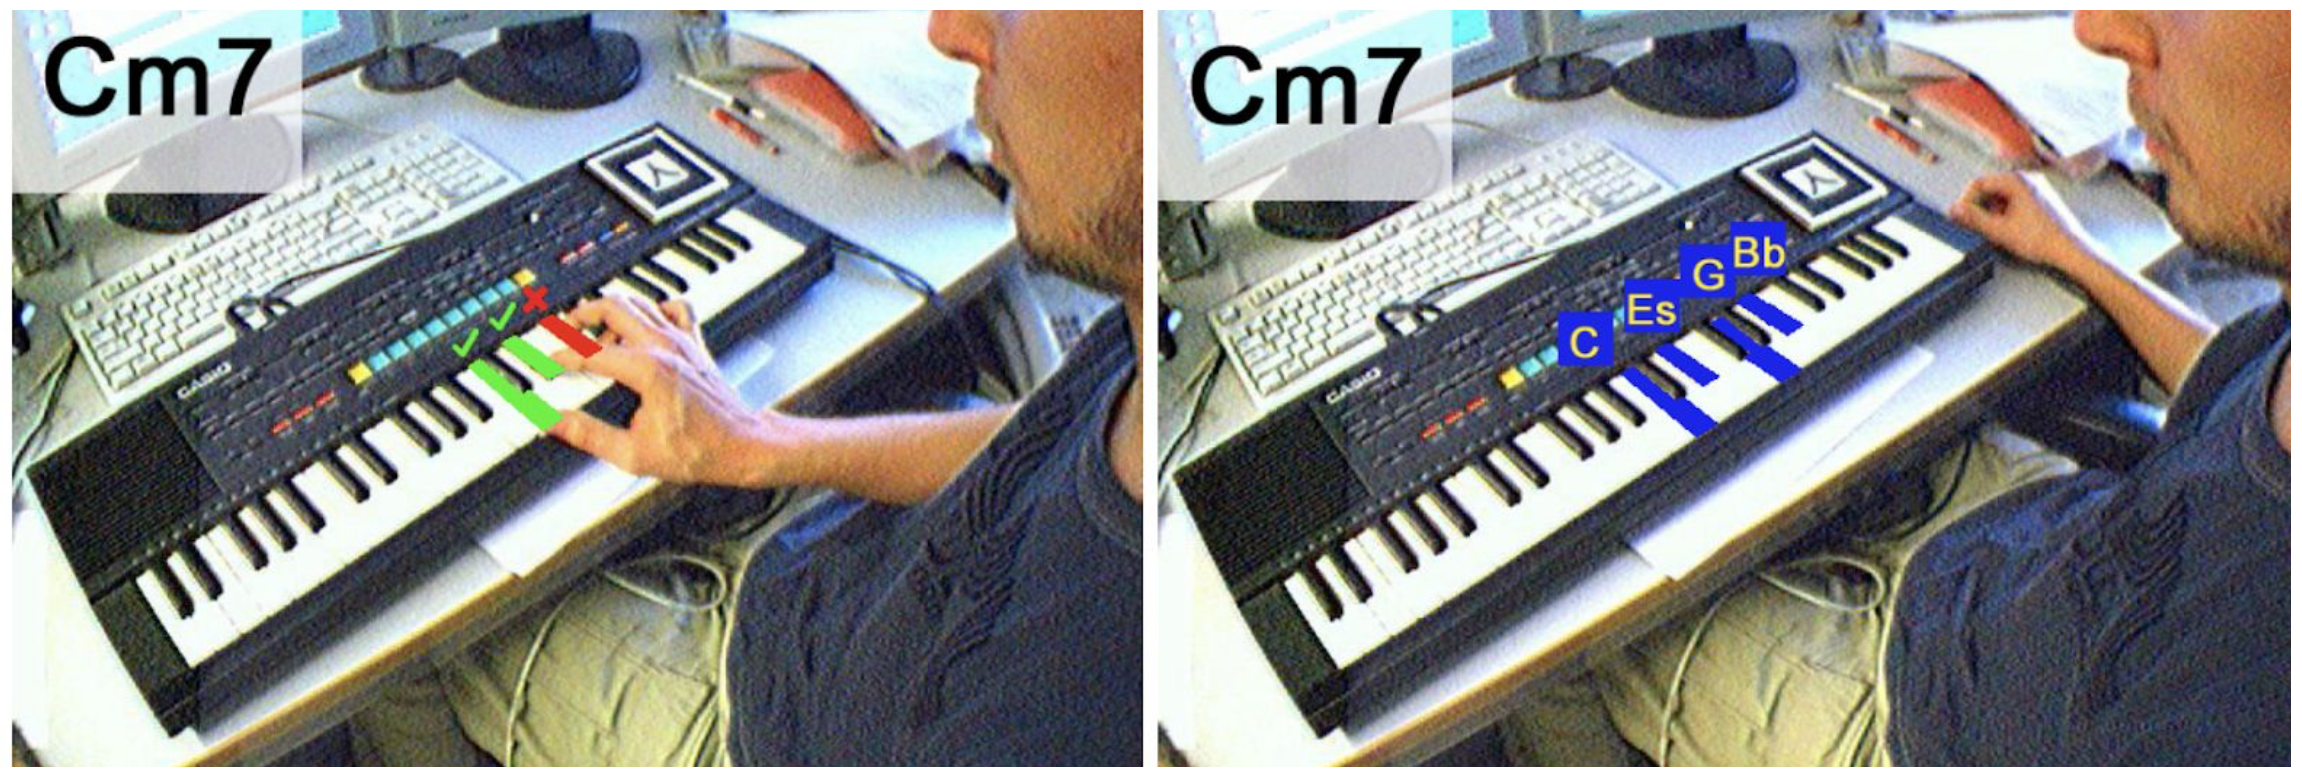
\includegraphics[width=12cm]{figures/barakonyi.png}
    \caption{Prototype by Brakonyi. Visualisations are seen overlying the keys of the MIDI keyboard.
    }\label{fig:barakonyi}
\end{figure}

Computer assisted music teaching systems date back to the early 2000’s. Here we present a couple of examples using XR environments. 

\begin{figure}[h]
\centering
 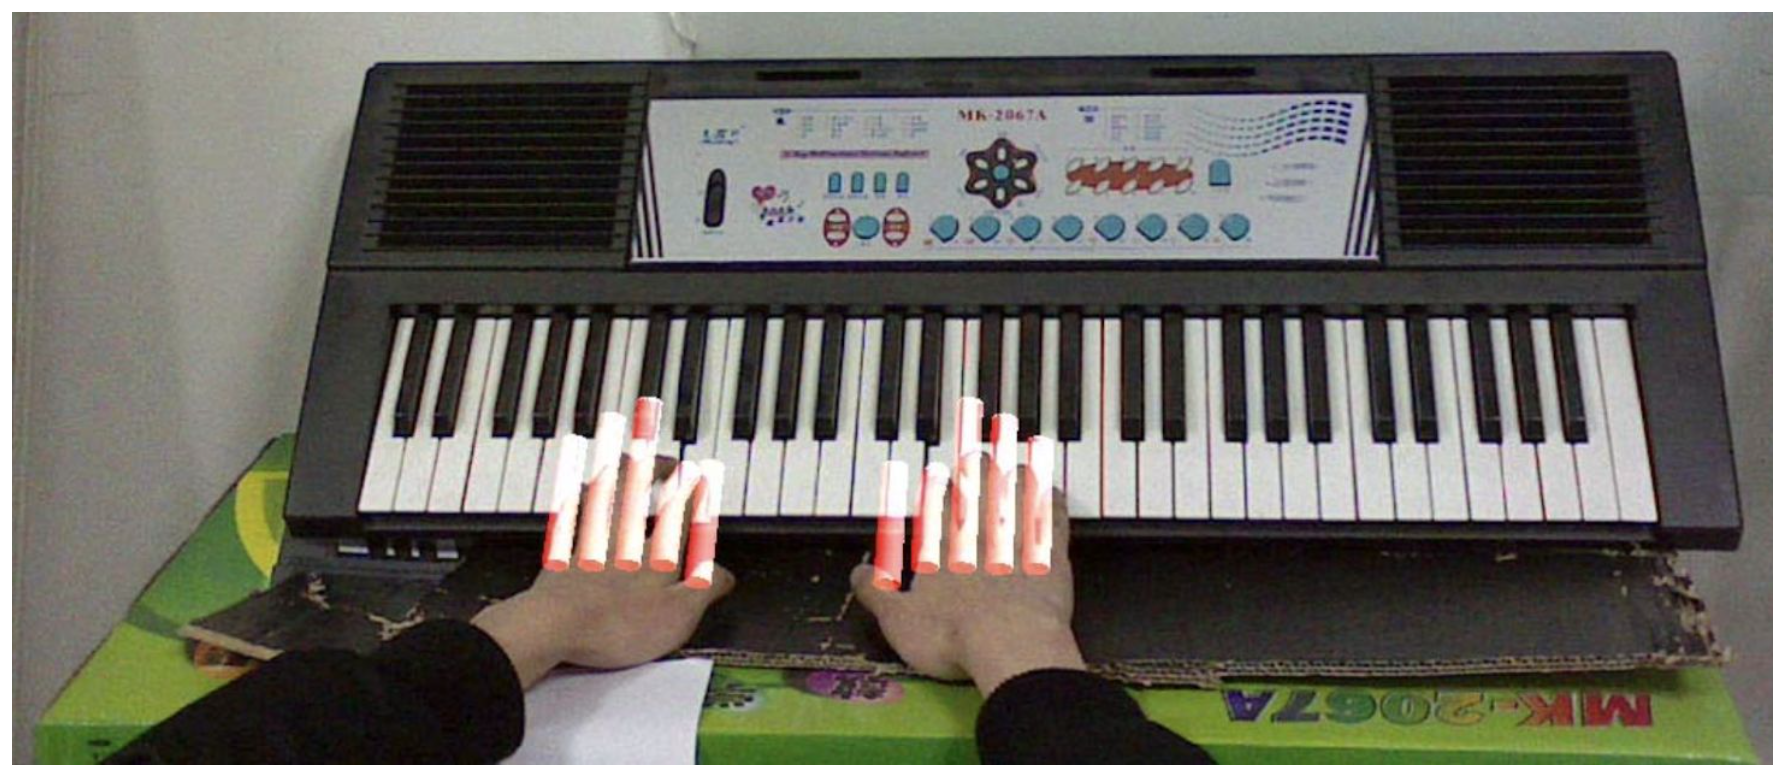
\includegraphics[width=12cm]{figures/huang.png}
    \caption{Prototype by Huang. The virtual hands are seen as overlaid the fingers and keys on the keyboard.
    }\label{fig:huang}
\end{figure}
\begin{figure}[h]
\centering
 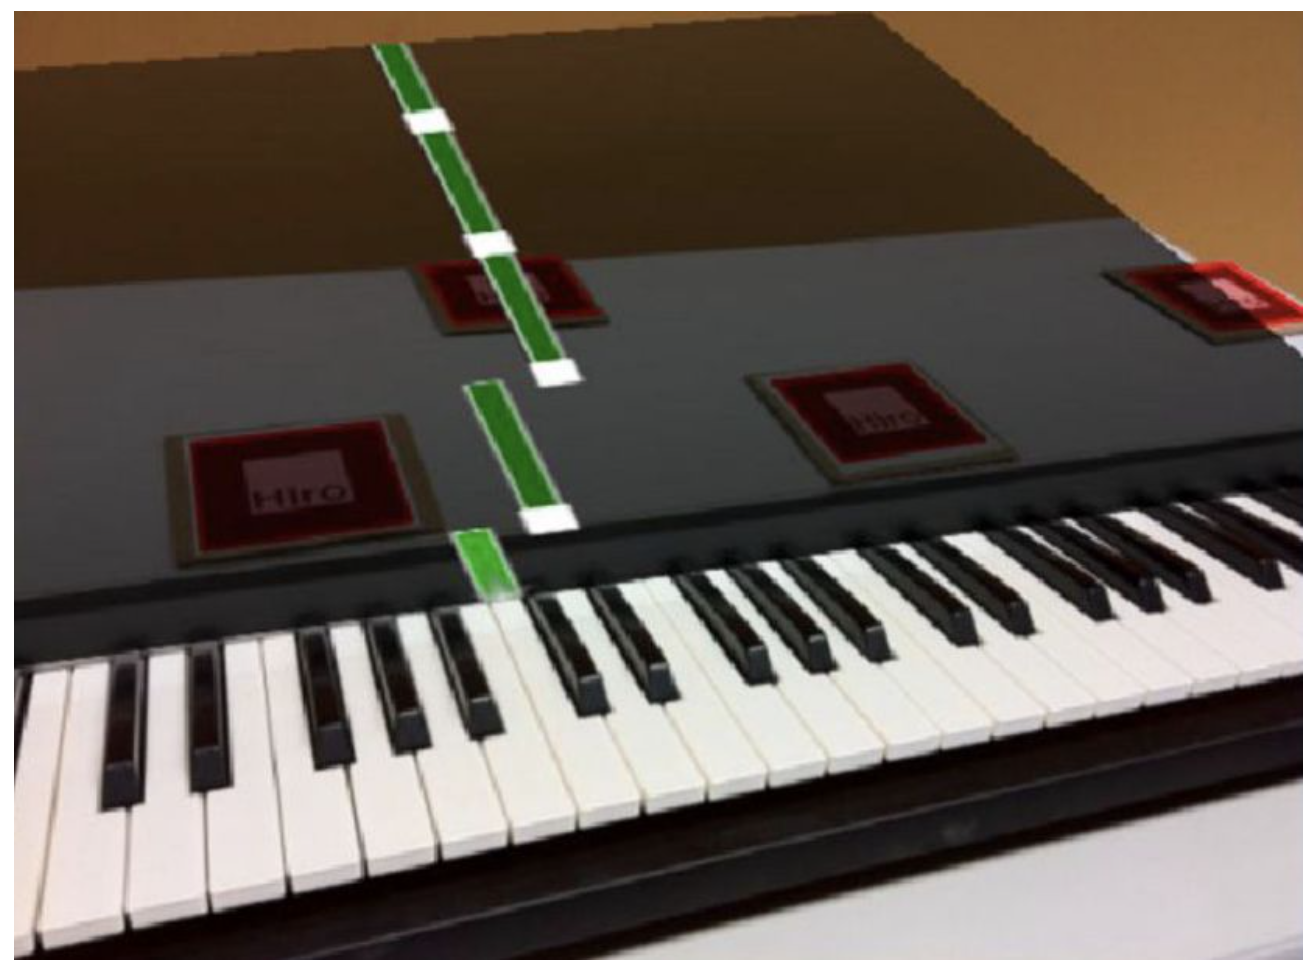
\includegraphics[width=12cm]{figures/chow.png}
    \caption{Prototype by Chow. A piano roll visualisation is seen as “falling notes” in the visualisations.
    }\label{fig:chow}
\end{figure}

\begin{itemize}
\item The work of \citet{barakonyi2005augmented} presented an AR piano tutor seen in Figure \ref{fig:barakonyi}. The prototype used a webcam, a monitor and a MIDI keyboard. The webcam captured the keyboard that was shown on the monitor together with digital information instructing users to hit certain keys in a defined order as well as giving audio feedback as to which keys have been pressed correctly and which were pressed by mistake. The system also included an advanced music composition tool by analysing the tunes currently being played and suggesting background chords and appropriate solo melodies. This technology allows it to understand its users but do not consider other factors such as cognitive load and spatiotemporal pointing data. 
\item The prototype of \citet{huang2011piano} presented a markerless AR based piano teaching system. It used virtual hands overlaid on a real keyboard (Figure \ref{fig:huang}), which allowed the beginners to practice playing the piano. The technology presented in this paper focused on the technological aspects of tracking the real keyboard and overlying virtual hands over the keys. The visualisations used in this prototype did not consider spatiotemporal pointing data. 
\item The paper by \citet{chow2013music} presents an AR prototype using a head mounted display. The prototype is targeting people who practice the instrument on their own (how it is done traditionally) and lack feedback on how to improve their playing as well as motivation for learning. Their prototype addressed these two shortcomings by visualising ``falling'' notes as seen in Figure \ref{fig:chow}} providing direct feedback, and including game elements to learning. The findings show that beginners improved their notation literacy. While the visualisations were effective, we believe that this can be improved further by considering pre-built user models. 
\item The work of \citet{weing2013piano} presents a prototype that enhances musical instrument learning with projected visualisations. Their P.I.A.N.O. prototype (Figure \ref{fig:ubicomp}) aims to support learning to play a piano by considering the learning curve of beginners and addressing hard-to-learn music notations. These notations are replaced by an alternative representation, which are projected onto the piano. Aside from the design of a piano prototype with interactive visualisations and projections, their study also proposed three different learning modes that support novice learners (listen, practice, play modes). They were able to improve on top of the work of \citet{chow2013music} by using gamification and interactivity to prolong student motivation. The P.I.A.N.O. was improved further in \cite{rogers2014piano} by mapping the correct visualisations with extra articulation or enhanced piano roll notation as referred to by authors. Their findings measured (i) significantly lower cognitive load, (ii) improved user experience, and (iii) an increase in perceived music quality rated by the experts as compared against non-projected piano roll notation. 
\end{itemize}
\begin{figure}[h]
\centering
 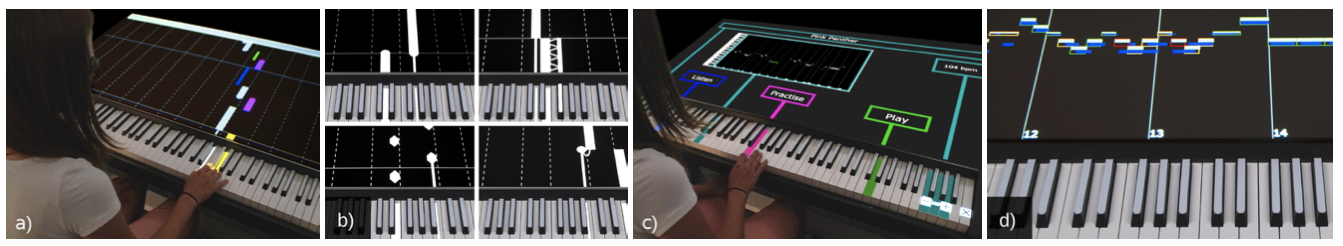
\includegraphics[width=12cm]{figures/pianoUBC.png}
    \caption{Photos of the P.I.A.N.O. interface by Rogers. It included overlaid visualizations, practice modes and detailed feedback. 
    }\label{fig:ubicomp}
\end{figure}

Most of the recent contributions in AR music teaching systems focus on either (1) introducing novel interfaces \cite{barakonyi2005augmented, huang2011piano}, (2) different learner modes for the users \cite{weing2013piano, rogers2014piano}, or (3) improving graphical rendering of the visualisations \cite{chow2013music, zheng2013general}. None of them took users’ cognitive load and response times into account, and were not based on the pre-built spatiotemporal pointing models in order to better support piano learning processes based on users’ performance. Our research will fill this gap by designing spatiotemporal-aware visualisations based on the pre-built models that take user-data into account, which will in our opinion improve AR piano learning experiences.\\

\section{Research Plan and Research Method}
\label{sec:plan}
The focus of this research will be on exploring AR piano systems anchored on the general research question: \textit{"How to support piano learners with adaptive visualizations based on novice and expert spatiotemporal models and cognitive load"}? The spatiotemporal models will allow us to understand the differences between the way experts and novices use the piano. By considering cognitive load, we can draw insights on how to design better visualizations. The specific research questions and the research plan are presented in the following subsections. 

\subsection{Research Questions}
Our research is guided by the following research questions: 
\begin{itemize}
    \item \textbf{RQ0: What other technological interventions that have been introduced to support piano learning?}\\
    Hypothesis: We believe that AR has been an effective piano learning supporting technology. However, in order to proceed with the succeeding RQ's we also need to survey and review the landscape of technology that support piano learning. By doing this, we can draw more inspirations towards better designing adaptive visualizations beyond the scope of AR. 
    \item \textbf{RQ1: Can we build a pointing model for adaptive visualizations in AR piano?} \\
    Hypothesis: We predict that based on the success of earlier studies on spatiotemporal pointing in AR, models of expert and novice usage can also be used to build adaptive visualizations to support piano learning. 
    \item \textbf{RQ2: Can we better support learners using spatiotemporal and cognitive load models?}\\
    Hypothesis: We believe that if we consider both spatiotemporal data and cognitive load of novices, we can better support their learning experiences \cite{rikers2004cognitive}.  \citet{lee2016website} states that determining the appropriate level of difficulty in game design is essential to ensure player experiences in an environment. By predicting error rates from player’s activities and measuring how overwhelmed they are using cognitive load, we could better support learning experiences in general. We believe that the same should be true in learning to play musical instruments.
    \item \textbf{RQ3: How do novices learn in AR piano under different learning conditions?}\\
    Hypothesis: Novices progress differently if they use adaptive visualisations that guide them in an AR piano prototype. We will explore the effects of adaptive visualizations in the long term learning of piano novices. 
    \item \textbf{RQ4: Can we adapt (or extend) these models to other musical instruments?}\\
    Hypothesis: Music teaching systems that use other instruments (like guitar or xylophone) possess the same elements and conditions required to observe and investigate spatiotemporal pointing. We predict that we can build multi-level (novice, intermediate and expert) models for these systems following the approach we did with the AR piano teaching system. If the later will prove successful we are sure the principles will work for other instruments and provide evidence for the hypothesis. 
\end{itemize}
\subsection{Method}
This research plan will have five (5) distinct phases leading to potential publications based on the intended contribution. These phases are namely, (1) Explore, (2) Model, (3) Augment, (4) Assess and (5) Extend. These phases have been mapped with the RQ's above and are described below: 
\begin{itemize}
    \item \textbf{Explore}: Survey of Piano Learning Support Technologies\\
    Publication title: Revisiting AR Piano Projection\\
    Target venue: UbiComp or ISS (demo paper) and/or DIS (provocation paper) and/or Creativity and Cognition (poster)
    \item \textbf{Model}: Understanding Novice and Expert Motion\\
    Publication title: A Pointing Model for Piano Roll Visualizations in Augmented Reality\\
    Target vene: CHI (full paper)
    \item \textbf{Augment}: Understanding Novice and Expert Workload\\
    Publication title: Supporting Novice Music Learners with Dynamic AR Feedback based on Cognitive Load\\
    Target venue: ICMI or UIST (full paper)
    \item \textbf{Assess}: Evaluating how novices learn in AR piano under different learning conditions\\
    Publication title: P.I.A.N.O. 2.0: Supporting Novice Piano Learning using Dynamic AR Feedback\\
    Target venue: ISMAR (full paper)
    \item \textbf{Extend}: Expanding the use of spatiotemporal models in AR music\\
    Publication title: Dynamic AR Feedback using Spatiotemporal Models for Learning Musical Instruments\\
    Target venue: CSCW (full paper)
\end{itemize}

\begin{table}[H]
\centering
\caption{Gantt Chart. One "*" represents one month in a quarter. } % removed vspace % add \textbullet ~
\begin{tabular}{|l|l|l|l|l|l|l|l|l|l|l|l|l|}
    \hline
    \multirow{\textbf{2020-2023}} & \multicolumn{2}{|c}{\textbf{2020}}&\multicolumn{4}{|c}{\textbf{2021}}&\multicolumn{2}{|c|}{\textbf{2022}}
    \\ \cline{2-9}& Q3    & Q4    & Q1    & Q2    & Q3     & Q4   & Q1  & Q2\\ \hline
    \textbf{Explore} & ***   &       &       &       &       &       &       &    \\ \hline
    \textbf{Model}   &       & ***   & ***   &       &       &       &       &    \\ \hline
    \textbf{Augment} &       &       &       & ***   &       &       &       &    \\ \hline
    \textbf{Assess}  &       &       &       &       & ***   & ***   &       &    \\ \hline
    \textbf{Extend}  &       &       &       &       &       &       & ***   & ***\\ \hline
\end{tabular}
\label{tab:ganttChart}
\end{table}

In \textbf{Explore}, we review existing prototypes and modalities that support teaching and learning piano. This phase will include focus group discussions (FGD), literature review and prototype design. The FGD involves the combined insights of HCI and UX practitioners who \textit{know how to design systems}, and piano players who \textit{know how to use the piano}. A systematic literature review will also be done on a set of AR piano prototypes introduced within the last 15 years. The \textbf{P.I.A.N.O.} prototype by \citet{rogers2014piano, weing2013piano} will be redesigned and built (temporarily called \textbf{PIANO 2.0}) following the insights from the FGD and the findings from the literature review. Novices will then be invited to train using PIANO 2.0 in order for us to know if this is a more preferred approach than the traditional setup. An open-source documentation of the project will also be shared. This phase will last around 3 months.  \\

In \textbf{Model}, we will investigate how spatiotemporal component of music in AR systems affects novice learning. We will invite at least 12 novices and another 12 expert participants to help us build spatiotemporal models of their movements and patterns while using PIANO 2.0. This will allow us to analyze and predict their error rates which we will then use to build adaptive visualizations. We will then validate our model and our adaptive visualizations in another user study with a new set of participants (at least 12 novices and 12 experts). We hope to reveal distinctions in the way novices and experts move when given visual stimuli that represents different piano chords. This will also allow us to analyze and categorize piano chords based on their temporal features. This phase is expected to last for about 6 months. \\

In \textbf{Augment}, we will investigate how cognitive load has an effect on the spatiotemporal performance of AR piano learners. We will invite 6 novices and 6 experts to help us build our cognitive load corpus. We will capture their electrocardiogram (ECG) and galvanic skin response (GSR) data in order to gauge their cognitive load. Using this, we will design dynamic AR feedback that adapts to both psycho cognitive and spatiotemporal responses. In a separate validation study, will attempt to find a relationship between changes in their emotional responses and their rate of errors while using our new visualization. We intend to uncover findings that will allow us to set guidelines in designing visual feedback that responds to the user's cognitive signals. Following the successes of \textbf{Explore} and \textbf{Model}, the \textbf{Augment} phase will last around 3 months. \\

In \textbf{Assess}, we will explore how adaptive visualizations contribute to long-term novice learning experiences. We will invite at least 12 novice participants to learn using our PIANO 2.0 prototype following a between-subject study design. The participants will be exploring three modes of adaptive visualizations that will provide live feedback and performance evaluation. These modes are (1) spatiotemporal adaptive visualizations, (2) cognitive load adaptive visualizations and (3) adaptive visualizations following both spatiotemporal and cognitive load models. The participants will be using PIANO 2.0 for multiple, succeeding sessions. We will measure if there is an improvement in terms of user experience and cognitive load. The recordings and outputs of the participants will also be assessed in a separate study with the help of at least 6 experts who will give their rating. This phase is expected to last for about 6 months. \\

In \textbf{Extend}, we will explore the spatiotemporal component of AR guitar, violin and xylophone projection systems. We will build adaptive visualizations that will work for musical instruments other than the piano. We will also explore the cognitive load and its effects for these musical instruments. We will use the same variables used in phases \textbf{Model} and \textbf{Augment} in building the models (error rates, cognitive load) and designing these adaptive visualizations. We will have a separate validation study that will explore how these users collaborate and manage different pacing levels. We will also look at how easy or difficult it is for novices to switch between music instruments given these adaptive visualizations. Following the successes of \textbf{Explore}, \textbf{Model}, \textbf{Augment} and \textbf{Assess}, the \textbf{Extend} phase will last around 6 months. \\
\section{Contributions}
\label{sec:contri}
We enumerate below the target contributions that the research aims to achieve: 
\begin{enumerate}
    \item spatiotemporal models of novices and experts pressing piano chords
    \item classification of chords in terms of complexity based on their temporal features
    \item adaptive visualizations for piano based on spatiotemporal models of users
    \item novice and expert cognitive load models while using AR piano systems
    \item relationship between spatiotemporal models (error rates) vs cognitive load of both novices and experts
    \item guidelines for adaptive visualizations based on cognitive load
    \item a comparative analysis of the effects to long term learning of the different adaptive visualizations
    \item improved UX and reduced cognitive load for users when using the AR piano
    \item validation of effectiveness and an improved music output based on expert evaluation
    \item spatiotemporal models of novice and experts on guitar, violin, xylophone, etc
    \item improved understanding of musical instruments based on temporal features
    \item guidelines towards multi-user collaboration coming from different mastery levels
\end{enumerate}

\begin{comment}
Most of the recent contributions in augmented reality music teaching systems focus on either (1) introducing a new ubiquitous interface, (2) having different learner modes for the users, and (3) improving graphical rendering of the visualizations. Studies that investigate and model spatiotemporal pointing on augmented reality music teaching systems are very limited. This will be the intended focus of this research. \\
We ask the general research question: “How might we model the interactions of experts and novices when using augmented reality music teaching systems and use them to design spatiotemporal-aware visualizations that can help novices in their music learning experiences?”. We use this general research question as the basis for our hypothesis statements. \\

We will model the spatiotemporal pointing activities of both novices and expert users while using an AR piano teaching systems. We believe that these models will allow us to understand the differences between the way experts and novices use these systems. With this, we will look into their patterns and the insights around them, which in turn we can use to design better visualizations. An overview of the research plan is described in Fig 4. The green branches show a set of experiments that aim to investigate the specific HCI application areas in relation to spatiotemporal pointing and augmented reality music teaching systems (piano, guitar, xylophone, etc). The orange branches show a range of setups that combine results from the experiments done in the green branches, and in relation to sensorimotor and psychophysics, bridging cognitive load and user models. Results of the experiments from the orange and green branches will provide groundwork for this research. The middle branch is the main focus of this thesis. It will focus mainly on augmented reality piano teaching systems. It will investigate the differences between the spatiotemporal models of novices and experts while using these systems. \\
\begin{landscape}
\begin{figure}[h]
\centering
 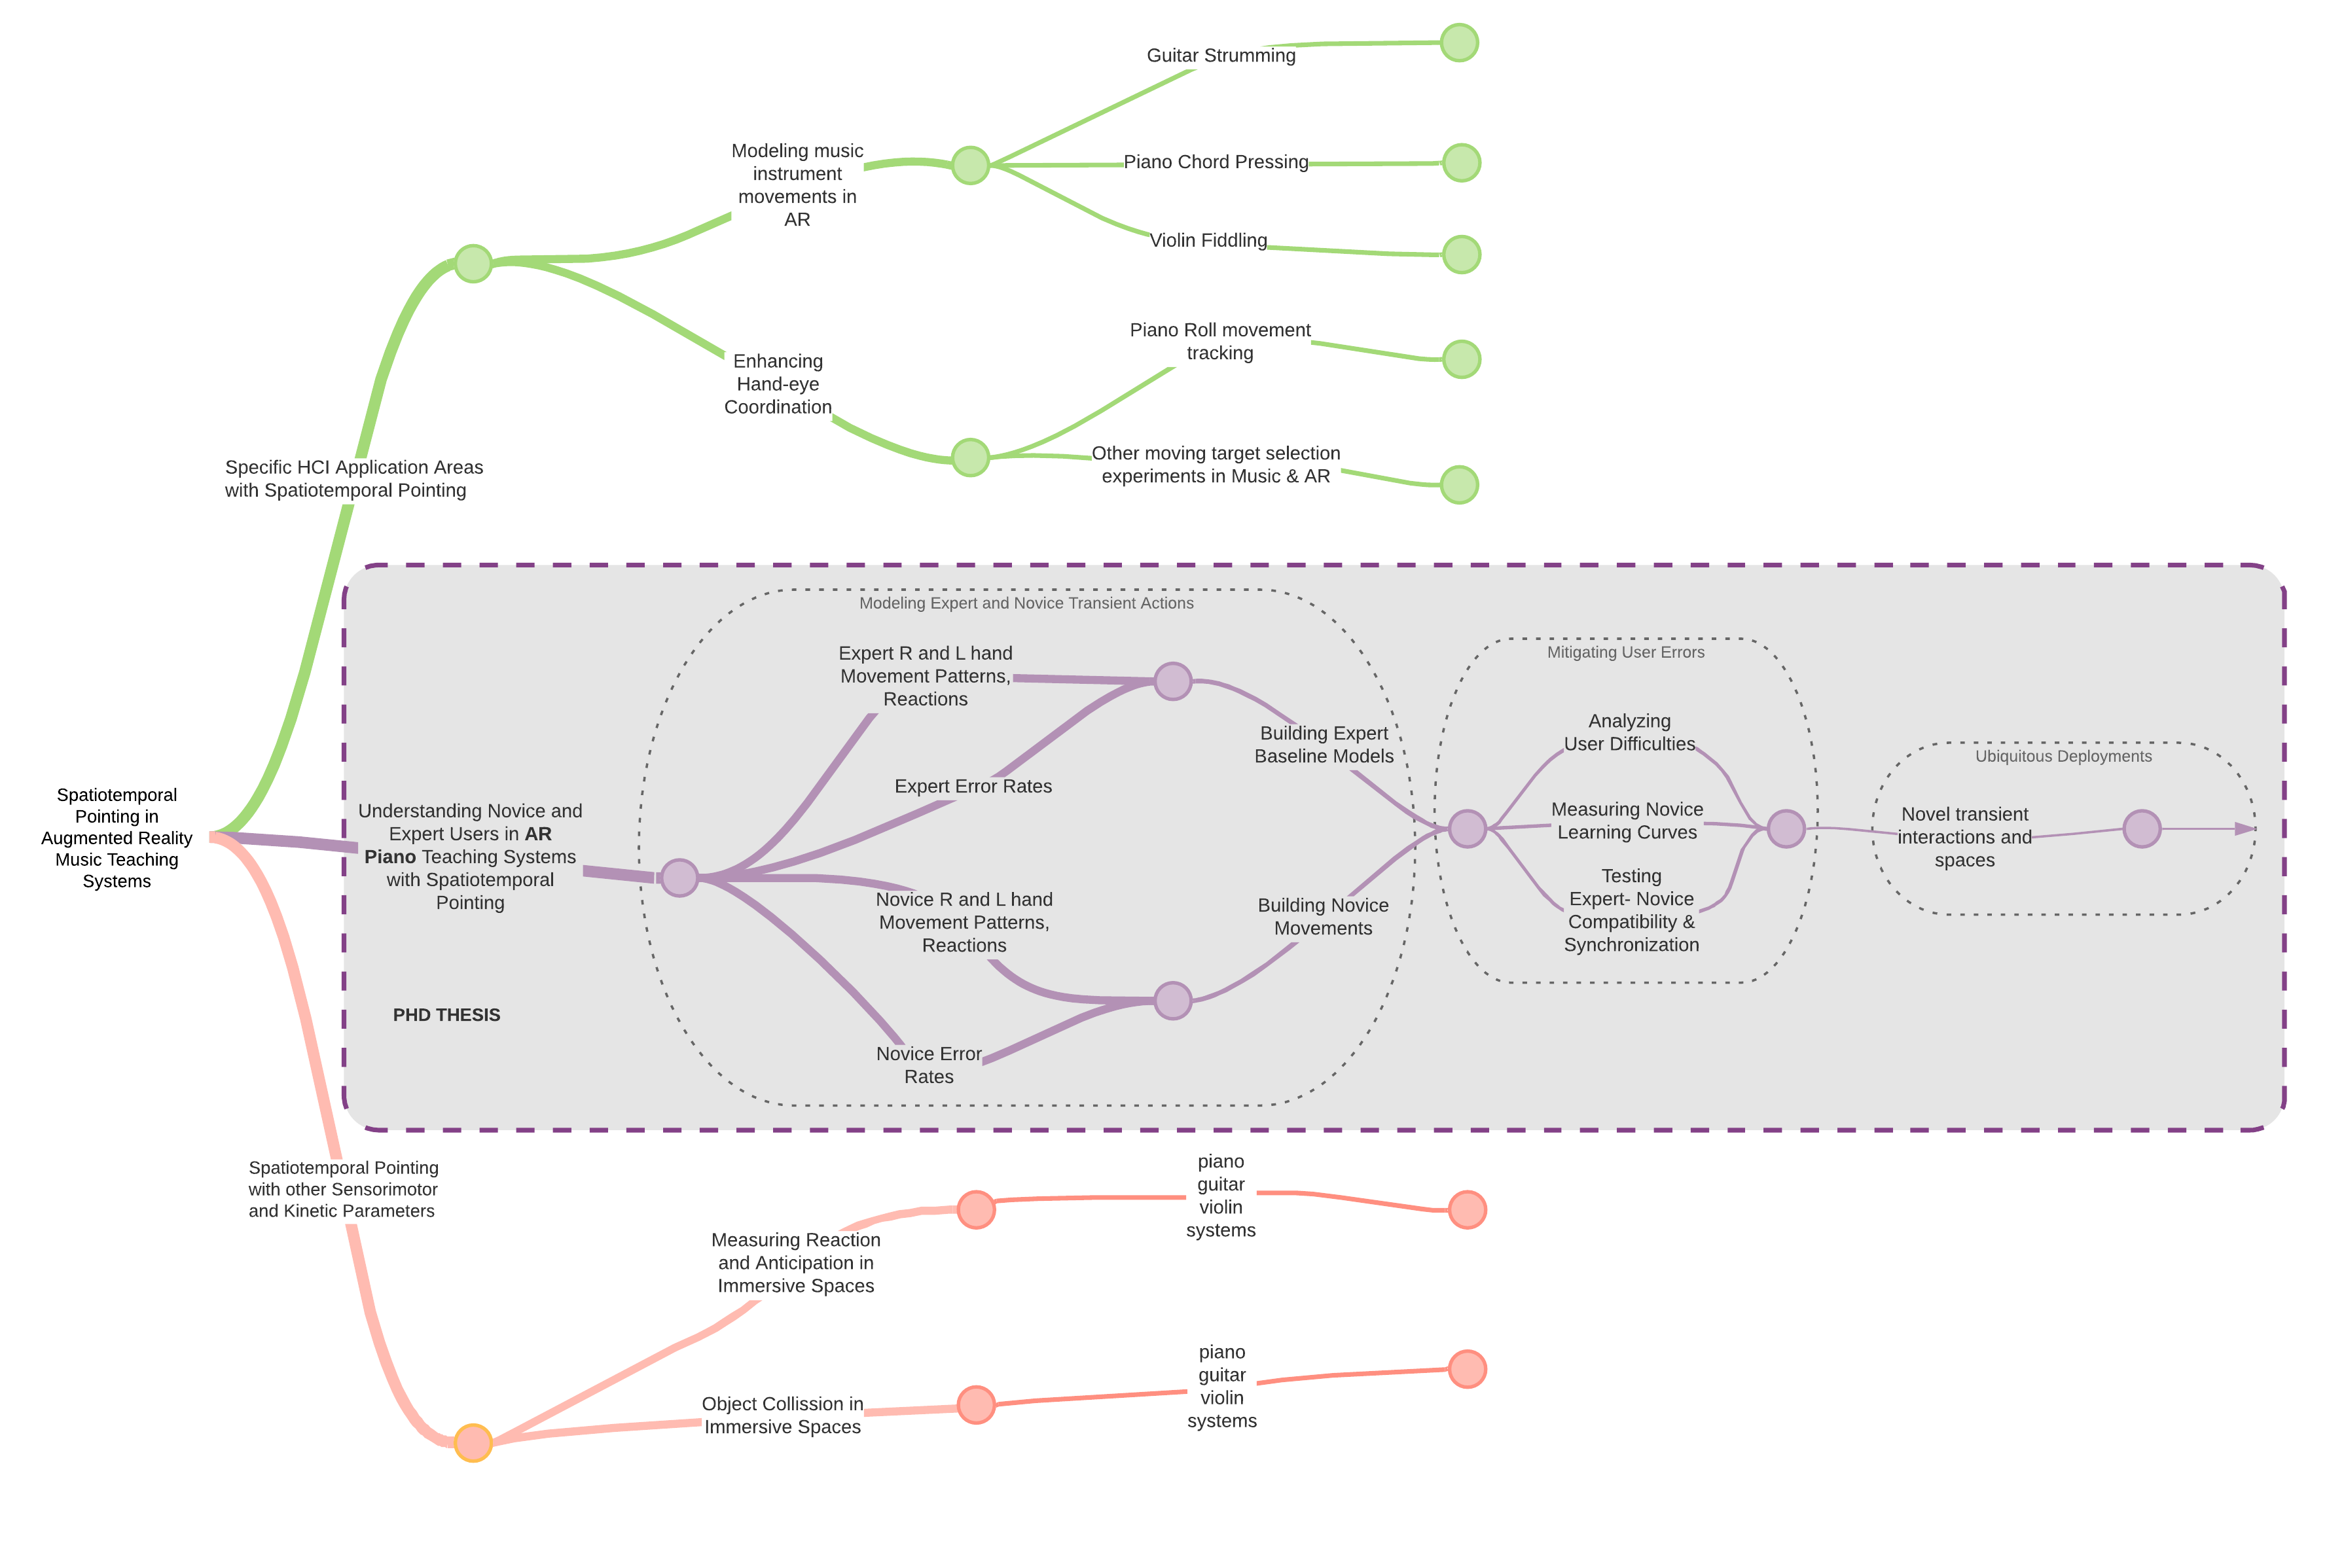
\includegraphics[width=\columnwidth\textheight]{figures/branches.png}
    \caption{An overview of the research branches showing breadth and depth. Each branch represents an experiment which will be part of the methodology in this proposal. Each node in the diagram is targetted  as a concrete contribution leading to a publication.
 }\label{fig:branches}
\end{figure}
\end{landscape}
\end{comment}


%%
%% The next two lines define the bibliography style to be used, and
%% the bibliography file.
\bibliographystyle{ACM-Reference-Format}
\bibliography{sample-base}
%%
%% If your work has an appendix, this is the place to put it.
%\appendix
\end{document}
\endinput
%%
%% End of file `sample-manuscript.tex'.
